\documentclass[10pt]{article}
\usepackage{acl}
\usepackage{times}
\usepackage{latexsym}
\usepackage[T1]{fontenc}
\usepackage[utf8]{inputenc}
\usepackage{microtype}
\usepackage{inconsolata}
\usepackage{enumitem}
\usepackage{url}
\usepackage{booktabs}
\usepackage{amsmath}
\usepackage{mathtools}
\usepackage{graphicx}
\usepackage{array}
\usepackage{xcolor}
\usepackage{tikz}
\usepackage{pgfplots}
\pgfplotsset{compat=1.17}
\usetikzlibrary{positioning, arrows.meta, shapes.geometric, fit, backgrounds, calc}

\setlist[itemize]{leftmargin=1.3em,itemsep=0.2em,topsep=0.2em,parsep=0em}
\urlstyle{same}

% Muted palette for the diagrams.
\definecolor{boxfill}{RGB}{245,245,245}
\definecolor{boxline}{RGB}{60,60,60}
\definecolor{accent}{RGB}{140,30,30}
\definecolor{soft}{RGB}{210,210,210}

% Default styles for the flow diagrams.
\tikzset{
  flowbox/.style={
    rectangle, rounded corners=2pt,
    draw=boxline, line width=0.4pt,
    fill=boxfill,
    minimum height=7mm, minimum width=18mm,
    align=center, font=\small, inner sep=3pt
  },
  flowbox-tall/.style={flowbox, minimum height=10mm},
  pillbox/.style={
    rectangle, rounded corners=4pt,
    draw=accent, line width=0.5pt,
    fill=white,
    minimum height=7mm, minimum width=20mm,
    align=center, font=\small, inner sep=3pt
  },
  flowarrow/.style={
    -{Latex[length=1.6mm]}, draw=boxline, line width=0.4pt
  },
  flowarrow-soft/.style={
    -{Latex[length=1.6mm]}, draw=soft, line width=0.4pt, dashed
  }
}

\title{ScholarRAG: A Trust-First Literature Assistant\\
with Sentence-Level Grounding and Calibrated Per-Citation Confidence}

\author{
Sushil Dalavi, Parvathi Sanjana Pericherla, Eshna Gupta \\
University of Southern California \\
\texttt{\{sdalavi, pperiche, eshnagup\}@usc.edu}
}

\begin{document}
\maketitle

\begin{abstract}
We built ScholarRAG to make literature-review answers easier to
verify, not just nicer to read. Every answer sentence is paired with
the specific passage it came from, and every citation gets a
calibrated confidence score made up of three signals: semantic match
between claim and passage, retrieval stability under query
paraphrases, and lexical corroboration across distinct sources. The
weights of that score are fit on 530 claim--evidence pairs
independently labeled by the three project authors. We do not
position the system as a competitor to general chatbots. It is a
narrow domain-trust layer for scholarly QA, and the main thing we
want to show is that this kind of interpretable per-citation
confidence can sit inside a working RAG system without slowing it
down. Source code, the labeled calibration set, and the full
evaluation pipeline are released
at \url{https://github.com/sushildalavi/CSCI-444/tree/main/Final_Project-ScholarRAG}.
\end{abstract}

%-----------------------------------------------------------------
\section{Introduction}
\label{sec:intro}

Most students we know already use ChatGPT or a similar tool for the
first pass of a literature review. The answers look good. The
problem is that you can rarely tell, without re-reading every paper,
whether the cited paper actually contains the claim that's been
attributed to it \citep{maynez2020faithfulness, rashkin2023attribution}.
The confidence numbers these tools sometimes show ($0.92$ confident,
$0.78$ confident) make things worse, not better. The same query gives
different scores on different runs, and the explanation behind the
score is rarely visible. So a polished answer ends up being trusted
because it sounds confident, not because the evidence is good.

ScholarRAG is our attempt to make that situation a little better. The
slogan we kept coming back to during the project was \emph{trust by
confidence, not by assertion}: the system should not tell you a claim
is supported, it should show you the passage and attach a calibrated
probability that the passage really does support the sentence. We
think this matters most for the people who are most exposed to
hallucinated citations: undergraduates, first-year graduate students,
and interdisciplinary researchers who have not yet built the muscle
to spot wrong citations on sight.

\paragraph{What we ended up with.}
The system has four ingredients that, together, are not standard in
RAG pipelines. First, citations are bound at the sentence level, not
at the paragraph or paper level. Second, each citation carries a
three-feature confidence score that we call \emph{M/S/A}: $M$ for
semantic match (an NLI-style entailment probability), $S$ for
retrieval stability under query paraphrases, $A$ for cross-source
lexical agreement. Third, the score is calibrated by a logistic
regression fit on labels we collected ourselves on the system's own
outputs, so the confidence numbers are not arbitrary heuristics.
Fourth, we are deliberately narrow: scholarly QA only. The narrowness
is what made the per-citation guarantees feasible to test.

\paragraph{Revision from the midterm report.}
After the midterm, the feedback was that the project read like a
generic RAG chatbot. We rewrote the framing around the trust angle,
made the three hypotheses explicit instead of implicit, and reported
human agreement \emph{before} calibration so the calibration result
is not floating on top of an unmeasured gold standard. This final
version is structured around those three hypotheses end to end.

%-----------------------------------------------------------------
\section{Background}
\label{sec:background}

Retrieval-Augmented Generation \citep{lewis2020rag} grounds an LLM in
documents fetched at query time instead of relying purely on
parametric memory. The standard recipe combines a dense bi-encoder
\citep{karpukhin2020dpr}, optionally a reranker
\citep{khattab2020colbert} or a fusion-in-decoder reader
\citep{izacard2021leveraging}, and a generator. The deployment shape
is almost always: retrieve top-$k$ chunks, drop them into a prompt,
ask the model for an answer with citations.

For scholarly QA we ran into three concrete problems with that
recipe. The first is that a citation in the answer does not actually
mean the cited passage supports the claim. Faithfulness work in
summarization and long-form generation has shown the same thing for
years \citep{maynez2020faithfulness, min2023factscore,
rashkin2023attribution}. The second is that the confidence numbers
people end up showing users are usually one of three things glued
together (retrieval similarity, generation likelihood, prompt
heuristics), and they tend to be overconfident
\citep{guo2017calibration, mahaut2024factual}. The third is that
RAG-style evaluation \citep{es2024ragas, zheng2023judging} happens
\emph{outside} the running system, so the user reading the answer
never sees those scores.

Three pieces of prior work were directly load-bearing for what we
built. NLI is a reasonable proxy for textual support
\citep{honovich2022true}, which is why $M$ is an entailment
probability rather than a similarity score. Predictive uncertainty
gets more honest when it is measured across runs or perturbations
\citep{lakshminarayanan2017simple, kuhn2023semantic}, which is what
$S$ is doing. Multi-evidence verification benchmarks
\citep{thorne2018fever} treat a claim corroborated by several
independent sources differently from one supported only once, which
is the intuition behind $A$. None of these signals is novel on its
own. The thing we have not seen done together is combining all three,
fitting their weights from human labels collected on the system's own
outputs, and rendering the result as a per-citation score in the same
UI as the answer.

%-----------------------------------------------------------------
\section{System}
\label{sec:system}

Figure~\ref{fig:overview} is a sketch of the deployed system. The
rest of this section walks through it.

\begin{figure*}[t]
\centering
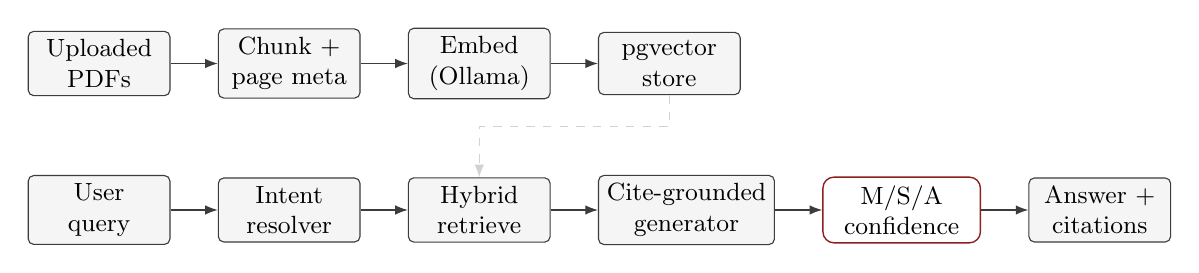
\begin{tikzpicture}[node distance=4mm and 6mm]
  \node[flowbox] (pdf)    {Uploaded\\PDFs};
  \node[flowbox, right=of pdf] (chunk) {Chunk +\\page meta};
  \node[flowbox, right=of chunk] (embed) {Embed\\(Ollama)};
  \node[flowbox, right=of embed] (store) {pgvector\\store};

  \node[flowbox, below=10mm of pdf] (q) {User\\query};
  \node[flowbox, right=of q] (intent) {Intent\\resolver};
  \node[flowbox, right=of intent] (retr) {Hybrid\\retrieve};
  \node[flowbox, right=of retr] (gen) {Cite-grounded\\generator};
  \node[pillbox, right=of gen] (msa) {M/S/A\\confidence};
  \node[flowbox, right=of msa] (ui) {Answer +\\citations};

  \draw[flowarrow] (pdf) -- (chunk);
  \draw[flowarrow] (chunk) -- (embed);
  \draw[flowarrow] (embed) -- (store);

  \draw[flowarrow] (q) -- (intent);
  \draw[flowarrow] (intent) -- (retr);
  \draw[flowarrow] (retr) -- (gen);
  \draw[flowarrow] (gen) -- (msa);
  \draw[flowarrow] (msa) -- (ui);

  \draw[flowarrow-soft] (store.south) -- ++(0,-4mm) -| (retr.north);
\end{tikzpicture}
\caption{End-to-end ScholarRAG. The top row is the offline ingest
pipeline (PDF $\rightarrow$ chunks $\rightarrow$ embeddings
$\rightarrow$ pgvector). The bottom row is the online query path: a
query is resolved, retrieved against the same store (dashed),
generated with sentence-level citations, scored on M/S/A, and
returned to the UI.}
\label{fig:overview}
\end{figure*}

\subsection{Ingestion and Hybrid Retrieval}
We parse uploaded PDFs into overlapping chunks with page metadata.
Chunks are embedded with \texttt{mxbai-embed-large} served by a local
Ollama instance, and the resulting vectors are written into a
PostgreSQL table with the \texttt{pgvector} extension. The slightly
unusual thing here is that every embedding row also stores a small
contract: provider, model, version, dimension. The retriever filters
on that contract at query time, which sounds finicky but is the
single change that has saved us the most pain. Long-running RAG
projects almost always end up with vectors from two different model
versions sharing one table, and those mixed-up neighborhoods are
hard to debug after the fact.

Retrieval itself is a hybrid: dense cosine over the embeddings, plus
a BM25-style lexical score, fused with $\alpha = 0.35$. We added
some balancing on top of the fusion so a single long paper does not
push everything else out of the candidate set. The same retriever
runs in two modes. In \emph{uploaded} mode it queries only the user's
own PDFs. In \emph{public} mode it fans out across OpenAlex, arXiv,
Semantic Scholar, Crossref, Springer, Elsevier, and IEEE, and then
deduplicates results by DOI and title fingerprint.

\subsection{Query Intent and Sense Disambiguation}
Short queries like \emph{transformer} or \emph{attention} are nasty,
because they mean different things in different fields. Before
retrieval, we send the query to GPT-4o-mini with a short timeout and
ask for a canonical term, an inferred domain, and a couple of search
variants. If that call fails or is disabled, we fall back to a small
hand-curated lexicon of ambiguous technical terms. We also reuse the
canonical term as a seed for the public APIs, which noticeably helps
recall on landmark papers whose titles do not contain the exact query
phrase.

\subsection{Citation-Grounded Generation}
Generation is GPT-4o-mini under a constrained prompt. The prompt
binds each output sentence to a specific provided passage and
explicitly tells the model to abstain or hedge when the evidence is
not enough, instead of synthesizing a new claim. After generation, a
short pass parses the inline citations, links them back to the chunk
identifiers used in retrieval, and runs an NLI entailment check per
sentence. Sentences that fail the check show up as weak in the UI.
Generation is not perfect, and that is exactly why the confidence
module is necessary.

\subsection{The M/S/A Confidence Model}

\begin{figure*}[t]
\centering
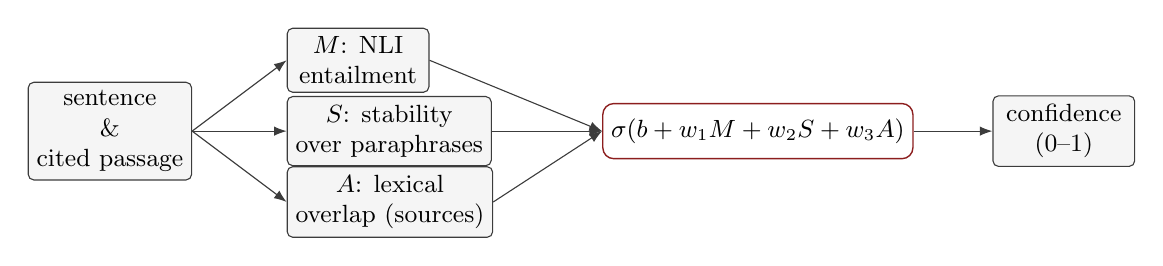
\begin{tikzpicture}[node distance=3mm and 8mm]
  \node[flowbox-tall] (pair) {sentence\\\&\\cited passage};
  \node[flowbox, right=12mm of pair, yshift=9mm]  (m) {$M$: NLI\\entailment};
  \node[flowbox, right=12mm of pair]              (s) {$S$: stability\\over paraphrases};
  \node[flowbox, right=12mm of pair, yshift=-9mm] (a) {$A$: lexical\\overlap (sources)};
  \node[pillbox, right=14mm of s] (sig) {$\sigma(b + w_1 M + w_2 S + w_3 A)$};
  \node[flowbox, right=10mm of sig] (out) {confidence\\(0--1)};

  \draw[flowarrow] (pair.east) -- (m.west);
  \draw[flowarrow] (pair.east) -- (s.west);
  \draw[flowarrow] (pair.east) -- (a.west);
  \draw[flowarrow] (m.east) -- (sig.west);
  \draw[flowarrow] (s.east) -- (sig.west);
  \draw[flowarrow] (a.east) -- (sig.west);
  \draw[flowarrow] (sig.east) -- (out.west);
\end{tikzpicture}
\caption{The M/S/A scoring path for one sentence--citation pair.
Three roughly independent signals are computed in parallel and then
combined through a logistic blend whose weights $(b, w_1, w_2, w_3)$
were fit on human labels.}
\label{fig:msa_pipeline}
\end{figure*}

For each sentence--citation pair we compute three numbers. $M$ is the
probability that the cited passage entails the sentence, obtained by
prompting GPT-4o-mini as a strict NLI classifier (with a token-overlap
fallback if the call breaks). $S$ is the fraction of perturbed
retrieval runs in which the same evidence is returned; the
perturbations are paraphrases of the original query, also from the
LLM. $A$ is the fraction of distinct source documents whose top
snippet shares at least two content words with the claim. We
intentionally kept $A$ a lexical signal rather than a second NLI
call. If $A$ used the same kind of inference $M$ does, the
calibration fit would partly be regressing the label on itself, and
the resulting weights would be misleading.

\begin{equation}
\widehat{\text{Confidence}}
= \sigma\!\bigl(b + w_1 M + w_2 S + w_3 A\bigr).
\label{eq:msa}
\end{equation}

The combined score is a plain logistic blend of the three features,
shown in Eq.~\ref{eq:msa}. We learn $(b, w_1, w_2, w_3)$ from
human-labeled pairs, described in Section~\ref{sec:methodology}. No
single feature is meant to capture evidence quality on its own; the
point of the blend is that the three failures modes are different
enough that combining them helps.

\subsection{Open-Corpus Annotation Loop}
The same system that serves answers can also export them. For any
query, the assistant writes one row per generated sentence, including
the query, the claim, the cited passage, and the precomputed $(M, S,
A)$ features. Three of us independently labeled each row as
\emph{Supported} or \emph{Unsupported} in identical workbooks. A
separate script computes pairwise Cohen's $\kappa$, takes a
majority vote across the three coders, and fits the logistic in
Eq.~\ref{eq:msa}. The winning weight row goes into a Postgres table.
At inference time, the production server loads the most recent
weights without a code change. The point of doing it this way is
that the calibration is not bolted to a specific benchmark. It can
drift with the corpus, and with the generator, over time.

\subsection{Stack}
React + TypeScript frontend (Vite). FastAPI backend in Python.
Postgres with \texttt{pgvector} for storage. Ollama for local
embeddings. GPT-4o-mini for intent resolution, generation, and the
NLI step inside $M$. The whole stack runs locally through Docker
Compose; we did not deploy to a cloud provider during the project.
The complete project source, including the backend services, React
frontend, database schema, and the calibration and evaluation
pipelines, is available at
\url{https://github.com/sushildalavi/CSCI-444/tree/main/Final_Project-ScholarRAG}.

%-----------------------------------------------------------------
\section{Experimental Methodology}
\label{sec:methodology}

\begin{figure}[t]
\centering
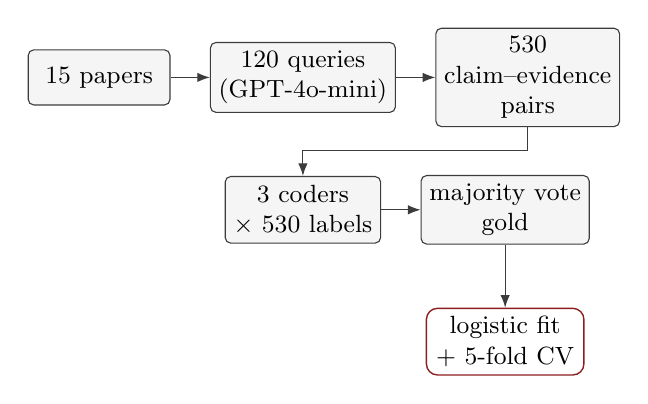
\begin{tikzpicture}[node distance=3mm and 5mm]
  \node[flowbox] (a1) {15 papers};
  \node[flowbox, right=of a1] (a2) {120 queries\\(GPT-4o-mini)};
  \node[flowbox, right=of a2] (a3) {530\\claim--evidence\\pairs};
  \node[flowbox, below=8mm of a2] (b1) {3 coders\\$\times$ 530 labels};
  \node[flowbox, right=of b1] (b2) {majority vote\\gold};
  \node[pillbox, below=8mm of b2] (b3) {logistic fit\\+ 5-fold CV};

  \draw[flowarrow] (a1) -- (a2);
  \draw[flowarrow] (a2) -- (a3);
  \draw[flowarrow] (a3.south) -- ++(0,-3mm) -| (b1.north);
  \draw[flowarrow] (b1) -- (b2);
  \draw[flowarrow] (b2) -- (b3);
\end{tikzpicture}
\caption{Evaluation pipeline. 15 landmark ML/NLP papers
$\rightarrow$ 120 queries across four query types $\rightarrow$ 530
sampled claim--evidence pairs $\rightarrow$ three independent human
labels per pair $\rightarrow$ majority-vote gold $\rightarrow$
logistic fit with stratified five-fold cross-validation.}
\label{fig:eval_pipeline}
\end{figure}

\subsection{Corpus and Queries}
The evaluation corpus is 15 landmark ML and NLP papers. The papers
span computer vision, generative modeling, reinforcement learning,
large language models, multimodal learning, computational biology,
and foundational ML. For each paper, we asked GPT-4o-mini for two
queries each in four query types: \emph{definitional},
\emph{methodology}, \emph{factual}, \emph{limitations}. That gives
$15 \times 4 \times 2 = 120$ evaluation queries. The four types are
not arbitrary: definitional queries are friendly to lexical
matching, methodology and limitations queries usually need
longer-context retrieval, and factual queries stress per-claim
grounding hardest.

\subsection{Three Hypotheses}
We organized the evaluation around three falsifiable claims.
\begin{itemize}
    \item \textbf{H1 (Faithful Confidence).} Higher
    $\widehat{\text{Confidence}}$ scores should mean the cited
    evidence really does support the generated claim more often. We
    test this with Brier score, AUC-ROC, and a reliability diagram.
    \item \textbf{H2 (Reliable Retrieval).} The hybrid retriever
    should land the target paper near the top of the retrieved set.
    We test this with Recall@$k$ and MRR, broken down by query type.
    \item \textbf{H3 (Trustworthy Gold).} Independent human coders
    should agree often enough that majority vote is a defensible gold
    standard for H1. We test this with pairwise Cohen's $\kappa$
    and the three-way unanimous agreement rate.
\end{itemize}

\subsection{Annotation Protocol}
The three human coders were the three project authors: Sushil
Dalavi, Parvathi Sanjana Pericherla, and Eshna Gupta. Each coder
independently labeled the same 530 claim--evidence pairs, sampled
with stratification on retrieval mode and query type so neither the
uploaded/public split nor the four query types were skewed. We
worked from identical workbooks. There was no AI judge in the loop,
and we did not discuss labels before submitting them. The single
binary task was: ``Does the cited passage adequately support the
generated claim?'' The three coder workbooks, the per-pair $(M, S,
A)$ feature table, and the majority-vote gold file are checked into
\texttt{Final\_Project-ScholarRAG/Evaluation/data/calibration} in
the project repository.

%-----------------------------------------------------------------
\section{Results}
\label{sec:results}

We present the three hypotheses in the order they validate the
system: trustworthy gold first (H3), then retrieval (H2), then
calibrated confidence (H1, which depends on H3).

\subsection{H3: The Gold Labels Are Trustworthy}

\begin{figure}[t]
\centering
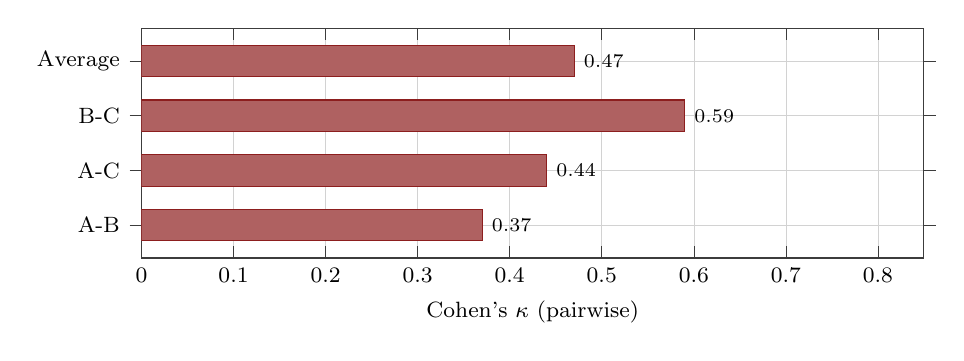
\begin{tikzpicture}
\begin{axis}[
    width=0.95\columnwidth, height=4.5cm,
    xbar,
    bar width=4mm,
    enlarge y limits=0.20,
    xmin=0, xmax=0.85,
    xlabel={Cohen's $\kappa$ (pairwise)},
    xlabel style={font=\footnotesize},
    symbolic y coords={A-B,A-C,B-C,Average},
    ytick=data,
    nodes near coords,
    nodes near coords style={font=\scriptsize, /pgf/number format/fixed, /pgf/number format/precision=2},
    tick label style={font=\footnotesize},
    axis line style={draw=boxline},
    tick style={draw=boxline},
    grid=major, grid style={draw=soft, very thin},
]
\addplot[fill=accent!70, draw=accent] coordinates {
  (0.37,A-B) (0.44,A-C) (0.59,B-C) (0.47,Average)
};
\end{axis}
\end{tikzpicture}
\caption{Inter-annotator agreement on the 530 labeled pairs. Average
pairwise Cohen's $\kappa = 0.47$, which is in the \emph{moderate}
band of the Landis--Koch scale. Three-way unanimous agreement is
$59.8\%$.}
\label{fig:iaa}
\end{figure}

Average pairwise Cohen's $\kappa$ across the three coders came out
at $0.47$ (Figure~\ref{fig:iaa}), which is in the moderate band of
the Landis--Koch scale. Three-way unanimous agreement was $59.8\%$,
on a label distribution that was almost balanced ($50.4\%$
supported, $49.6\%$ unsupported). Two readings come out of this. The
first is that binary support judgments are genuinely hard, even for
trained humans on this corpus, so the dataset is not a giveaway.
The second is that agreement is high enough that majority vote across
the three coders is a defensible gold standard for H1. We treat H3
as supported.

\subsection{H2: Retrieval Finds the Right Paper}

\begin{figure}[t]
\centering
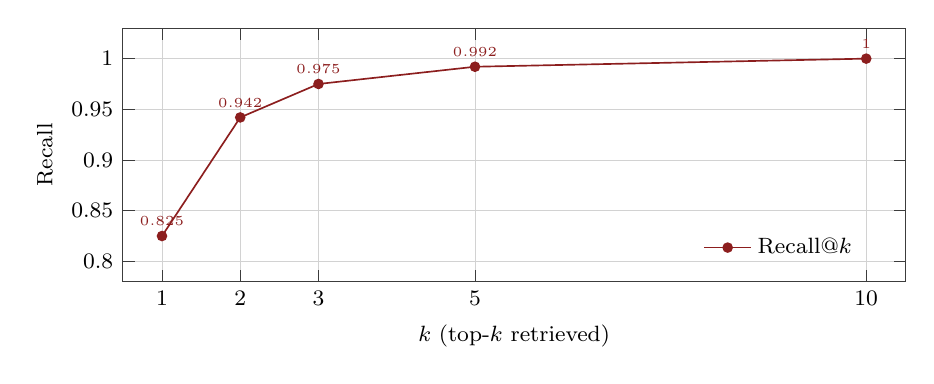
\begin{tikzpicture}
\begin{axis}[
    width=0.95\columnwidth, height=4.8cm,
    xlabel={$k$ (top-$k$ retrieved)},
    ylabel={Recall},
    xlabel style={font=\footnotesize},
    ylabel style={font=\footnotesize},
    tick label style={font=\footnotesize},
    xmin=0.5, xmax=10.5,
    ymin=0.78, ymax=1.03,
    xtick={1,2,3,5,10},
    ytick={0.80,0.85,0.90,0.95,1.00},
    grid=major, grid style={draw=soft, very thin},
    axis line style={draw=boxline},
    tick style={draw=boxline},
    nodes near coords,
    nodes near coords style={font=\tiny, /pgf/number format/fixed, /pgf/number format/precision=3},
    every node near coord/.append style={anchor=south},
    legend style={font=\footnotesize, draw=none, fill=none, at={(0.95,0.05)}, anchor=south east},
]
\addplot[mark=*, mark size=1.6pt, color=accent, line width=0.6pt]
  coordinates {(1, 0.825) (2, 0.942) (3, 0.975) (5, 0.992) (10, 1.000)};
\addlegendentry{Recall@$k$}
\end{axis}
\end{tikzpicture}
\caption{Closed-loop retrieval on the 120 generated queries against
the 15-paper corpus. Recall climbs from $0.825$ at $k=1$ to $0.992$
at $k=5$ and saturates at $1.000$ at $k=10$. MRR is $0.981$.}
\label{fig:recall}
\end{figure}

The closed-loop sanity check on the 120-query benchmark put the
target paper in the top-5 on $99.2\%$ of queries and in the top-10
on every single one (Figure~\ref{fig:recall}); MRR is $0.981$. The
breakdown by query type is what we expected: definitional, factual,
and limitations queries hit Recall@5 = 1.00, while methodology
queries land at $0.97$. Methodology was the hardest because the
target evidence is often a procedure description spread across
several pages instead of a single dense paragraph. We treat H2 as
supported.

\subsection{H1: Confidence Is Faithful}

\begin{figure}[t]
\centering
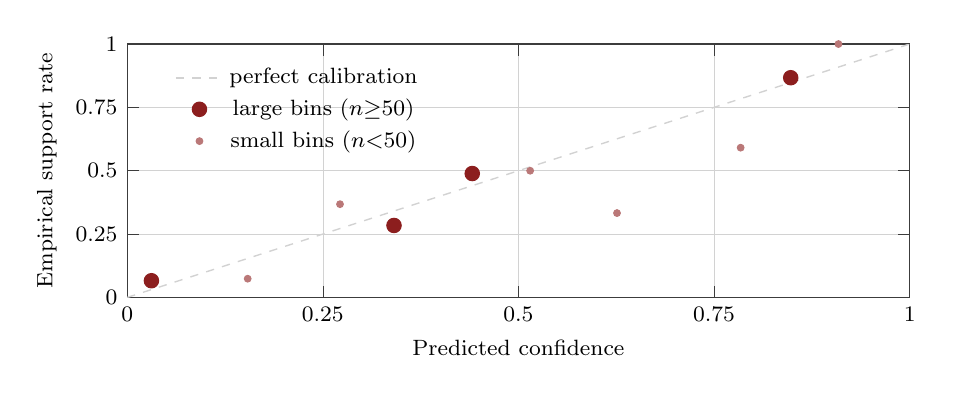
\begin{tikzpicture}
\begin{axis}[
    width=0.95\columnwidth, height=4.8cm,
    xlabel={Predicted confidence},
    ylabel={Empirical support rate},
    xlabel style={font=\footnotesize},
    ylabel style={font=\footnotesize},
    tick label style={font=\footnotesize},
    xmin=0, xmax=1, ymin=0, ymax=1,
    xtick={0,0.25,0.5,0.75,1.0},
    ytick={0,0.25,0.5,0.75,1.0},
    grid=major, grid style={draw=soft, very thin},
    axis line style={draw=boxline},
    tick style={draw=boxline},
    legend style={font=\footnotesize, draw=none, fill=none,
                  at={(0.05,0.95)}, anchor=north west},
]
\addplot[domain=0:1, samples=2, dashed, color=soft, line width=0.5pt] {x};
\addlegendentry{perfect calibration}
\addplot[only marks, mark=*, mark size=2.6pt, color=accent]
  coordinates {
    (0.031, 0.066) (0.341, 0.284) (0.441, 0.489) (0.848, 0.867)
  };
\addlegendentry{large bins ($n{\geq}50$)}
\addplot[only marks, mark=*, mark size=1.2pt, color=accent!60]
  coordinates {
    (0.154, 0.074) (0.272, 0.368) (0.515, 0.500)
    (0.626, 0.333) (0.784, 0.591) (0.909, 1.000)
  };
\addlegendentry{small bins ($n{<}50$)}
\end{axis}
\end{tikzpicture}
\caption{Reliability diagram of the calibrated confidence on 530
gold-labeled pairs. Brier $=0.160$ and AUC-ROC $=0.852$ on the
full fit. The four large bins ($n \geq 50$, holding $438/530$ of the
pairs between them) sit close to the diagonal; the smaller bins are
noisier, which is what we would expect at $n$ in the single digits.}
\label{fig:h1}
\end{figure}

The fitted unified blend reaches Brier $=0.160$ and AUC-ROC
$=0.852$ on the full 530-pair fit, and the result is stable
under stratified five-fold cross-validation
(Figure~\ref{fig:h1}). The bin we care about most is the $0.85$
bucket: it holds $180$ of the $530$ pairs, and its empirical
support rate ($0.87$) is essentially on the diagonal. The other
high-mass bins ($n=76$ at $0.03$, $n=94$ at $0.44$, $n=88$ at
$0.34$) also track the diagonal closely. Bins with only a handful
of points are visibly noisier, but they hold a small fraction of
the pairs. We treat H1 as supported.

\paragraph{What the learned weights tell us.}
The fit puts most of the mass on $M$ and $A$, both with large
positive weights, and gives $S$ a small near-zero weight. We were
honestly expecting $S$ to do more work than it did. The reading we
ended up with is that, on this corpus, a passage that strongly
entails the claim is also the passage that recurs across paraphrased
queries. Once $M$ is in the model, $S$ adds very little new
information. We do not think this means stability is a bad signal in
general. We think it means our paraphrases were too mild to pull $S$
apart from $M$. That is a clean target for future work, not a
verdict on the framework.

\subsection{System in Action}
A typical session in uploaded mode looks like this. The user uploads
a paper, asks a question about it, and the answer appears with
inline citations, each one annotated with its M/S/A score. The
right-hand panel shows the actual sentences that supported each
citation. Follow-up questions stay grounded in the same evidence
pool. When no good evidence exists, the system abstains rather than
generating a confident-sounding hallucination, which was a hard
behavior to prompt for and one we are still tuning.
End-to-end median latency in uploaded mode is roughly half a second
at the FastAPI boundary, dominated by the LLM generation step.
Public mode is bounded by the upstream APIs and is several seconds
slower because it fans out to seven providers in parallel.

%-----------------------------------------------------------------
\section{Limitations}
\label{sec:limitations}

A few things this work does \emph{not} show.

\paragraph{The labeled set is small.}
Five hundred and thirty pairs is enough to fit a three-feature
logistic and stress-test it under cross-validation, but it is not
enough to rule out long-tail failures. Our queries are also generated
by GPT-4o-mini, not collected from real users. Real-world questions
will be vaguer, noisier, and more interdisciplinary than what we
tested on.

\paragraph{Retrieval is still hand-tuned.}
We use a hand-picked $\alpha$ and several balancing heuristics. They
work well on this benchmark, but none of them are learned. A learned
cross-encoder reranker on top of the existing fusion would almost
certainly improve the top-ranked result.

\paragraph{Sense disambiguation is narrow.}
The deterministic fallback lexicon only covers a small set of
ambiguous technical terms. The LLM-based intent resolver covers more,
but we have not evaluated its judgments against a held-out intent
benchmark, so we cannot characterize its failure modes well.

\paragraph{M/S/A is not a hallucination detector.}
If two papers are confidently wrong in the same way, $A$ rewards the
agreement and $M$ rewards the entailment, even though the underlying
claim is false. M/S/A measures \emph{evidential} support, not
\emph{factual} truth. The system is meant to help a human verify the
cited passages, not to replace expert judgment.

%-----------------------------------------------------------------
\section{Future Work}
\label{sec:future}

\paragraph{Stronger retrieval.}
The most direct next step is a learned cross-encoder reranker on top
of the dense + lexical fusion, plus a head-to-head against newer
embedding models. We expect this to close the residual gap on
methodology queries.

\paragraph{A larger, harder calibration set.}
We want to scale the annotation loop to several thousand pairs, with
deliberate over-sampling of borderline cases: paraphrased support,
partial support, off-topic but related evidence, and claims that are
true but not supported by the cited passage. We also want to push
$S$ harder by paraphrasing queries more aggressively, so that
retrieval stability becomes informative beyond what $M$ already
captures.

\paragraph{Better source pool.}
For public mode we plan to add reputable, domain-specific sources
(PubMed, ACL Anthology, NeurIPS proceedings) and improve
deduplication so that ``multi-source agreement'' actually means
several independent corroborations, not the same metadata record
repeated by different aggregators.

\paragraph{Open questions.}
Two questions came out of this work that we cannot answer with an
offline benchmark. First, can the M/S/A framework generalize past
literature review, to coding assistants, legal-research tools, or
medical QA, in a way that genuinely helps both informed and naive
users? Second, does sentence-level grounded confidence actually
change user behavior: do students click through to cited passages
more often, and do they appropriately lower their trust when the
score is low? Both questions need a user study, not another offline
metric.

%-----------------------------------------------------------------
\section{Conclusion}
\label{sec:conclusion}

The premise we started from is simple: an answer about research
papers should be easy to verify, not just easy to read. So we built
a literature assistant that grounds every answer sentence in a
specific passage, and attaches a calibrated per-citation confidence
score combining semantic match, retrieval stability, and lexical
agreement. The bigger point we wanted to make is that trust deserves
to be a first-class output of the system, on the same level as the
answer itself. A citation alone is not enough. A confidence number
alone is not enough. By combining sentence-level grounding,
human-calibrated confidence, and an open-corpus annotation loop,
ScholarRAG sketches what a literature assistant that is fluent,
fast, and easier to verify could look like in practice.

\bibliography{custom}
\bibliographystyle{acl_natbib}

\end{document}
